\documentclass[slantfont,boldfont]{ctexart}
\def\pgfsysdriver{pgfsys-dvipdfmx.def}
\usepackage[hmargin={20mm,20mm},vmargin={20mm,10mm}]{geometry}
\usepackage{indentfirst}
\usepackage{graphicx}

\begin{document}

\title{这是神马字体渲染?}
\author{比尔盖子}
\maketitle

很早以前,我成功配置了Wine的字体,非常漂亮,就像这样:
\begin{figure}[htbp]
    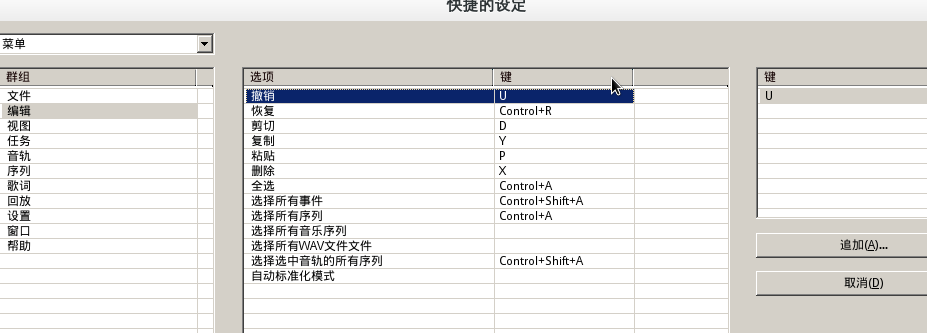
\includegraphics[width=12cm]{images/vocaloid-before.png}
    \centering
\end{figure}


配好字体真是太不容易了,于是,我赶紧备份了\verb|.wine|文件夹,以便日后直接恢复。后来,\verb|Wine|配置真的坏了,我就还原了备份的\verb|.wine|文件夹,结果发
现是同样的字体,但是渲染效果居然变成这样了……\\\\
\begin{figure}[htbp]
    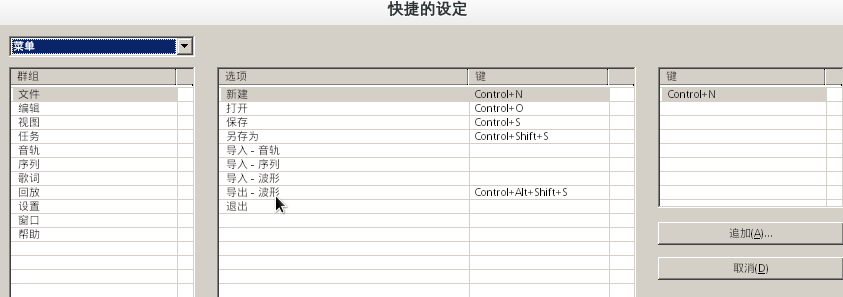
\includegraphics[width=12cm]{images/vocaloid-now.png}
    \centering
\end{figure}

\end{document}
